%%TODO:
%% Add goals - they are similar to \cite{1323562}, i.e.
%%      Examine multicore performance as compared to single core performance
%%      Expose bottlenecks to scaling up from one core to many cores
%%      Determine if the bottlenecks are application specific or not
%%      Suggest and attempt solutions
%%

%\documentclass{acm_proc_article-sp}
%\documentclass[pdftex,conference,letterpaper,10pt]{IEEEtran}
%\documentclass[times, 10pt,twocolumn]{article}
\documentclass[conference, compsoc]{IEEEtran}
\usepackage{latex8}
\usepackage{times}
%\usepackage[left=1in,top=1in,right=1in,bottom=1in]{geometry}
\usepackage{graphicx}
%\usepackage{psfrag}

%for PDF features - http://www.ce.cmu.edu/~kijoo/latex2pdf.pdf
%\usepackage[pdftex]{hyperref} % For the bookmark/hyperlinks
%%
%\hypersetup{%
%    pdftitle={Evaluating the Performance of Network Protocol Processing on Multi-core Systems},
%    pdfauthor={Matthew Faulkner, Andrew Brampton and Stephen Pink},
%    pdfkeywords={},
%    bookmarksnumbered,
%    pdfstartview={FitV},
%    colorlinks={false},  % No color links
%    pdfborder={0 0 0}   % No borders around links
%}


\begin{document}

\title{Evaluating the Performance of Network Protocol Processing on Multi-core Systems}
%\numberofauthors{3}

%\author{
%Matthew Faulkner, Andrew Brampton and Stephen Pink\\
%Computing Department\\ InfoLab 21\\ Lancaster University
%Lancaster, Lancashire, LA1 1SY\\ \}faulknem, brampton, pink\}@comp.lancs.ac.uk\\
%% For a paper whose authors are all at the same institution,
%% omit the following lines up until the closing ``}''.
%% Additional authors and addresses can be added with ``\and'',
%% just like the second author.
%
%}

\author{Matthew Faulkner, Andrew Brampton and Stephen Pink\\
Computing Department\\ Lancaster University,\\
 \{faulknem,brampton,pink\}@comp.lancs.ac.uk\\
% For a paper whose authors are all at the same institution,
% omit the following lines up until the closing ``}''.
% Additional authors and addresses can be added with ``\and'',
% just like the second author.
%\and
%Second Author\\
%Institution2\\
%First line of institution2 address\\ Second line of institution2 address\\
%SecondAuthor@institution2.com\\
}

\maketitle
\begin{abstract} % Max 200 words

Improvements at the physical network layer have enabled technologies such as 10 Gigabit Ethernet. Single core end-systems are unable to fully utilise these networks, due to limited clock cycles. Using a Multi-core architecture is one method which increases the number of available cycles, and thus allow networks to be fully utilised. However, using these systems creates a new set of challenges for network protocol processing, for example, deciding how best to utilise many cores for high network performance.

This paper examines different ways the cores of a multi-core system can be utilised, and, by experimentation, we show that in an eight core system deciding which cores to use is important. In one test, there was a 40\% discrepancy in CPU utilisation depending on which cores were used. This discrepancy results from the resources each core shares, an example being the multi-hierarchy CPU caches, and to which bus the processors are connected.
\hfill
\end{abstract}

\section{Introduction}
\label{sect:Intro}
The rapid growth of the Internet and improvements in distributed computing has made efficient communication an increasing concern to the network researcher. Research has continually improved the speed at which networks can transfer data. Advances in microprocessor performance have always allowed processors to match this increasing speed. However, as we approach the limits of uni-processor performance~\cite{agarwal00clock} new techniques are required within the end-host. Multi-core architectures have the potential to match the improvements made by the network.
%MF: AINA: Multi-core techniques are an advancement in microprocessor design which may continue to match network improvements.

Multi-core systems allow the network and application processing to be executed concurrently on different cores. %MF: AINA: on one or more cores.
Utilising multi-core systems therefore creates a new set of challenges for network protocol processing. One of these challenges, for example, is to decide which core should execute the application and which core should perform the network processing. When all the processing takes place on a single-core, only one core's clock cycles are available. If both the network processing and application processing are executed on different cores then the available clock cycles are increased. However, performance does not scale linearly with clock cycles because cores must contend for shared resources. Examples of these resources include system devices, such as network adaptors, and shared memory.

%Concurrency controls are needed when there is shared data or devices which may be accessed simultaneously. Locks are one synchronisation mechanism which limit concurrent access. A core must wait if a shared resource is currently in use by another core. Obviously, locks are not needed for this reason on uniprocessor systems. In most networking subsystems, there are two main categories of locks: global locks and connection based locks. The former provides protection across all global structures such as the socket table, as well as access to the networking hardware. The latter provides protection for per-connection-based data structures. Such locks are required by TCP, for example, to avoid simultaneous updates to the connection's sequence number.
%
%Main memory lookups take many CPU clock cycles. To improve memory performance, each CPU maintains a local cache of high speed memory. These caches hide the high latency caused by accessing main memory. Multi-core machines use multi-level cache hierarchies; typically, two levels of cache, one smaller, faster and closer to the processor than the other, but both faster and closer than main memory. Caches at each level may have different access latencies, memory sizes, and are shared by different sets of cores. To aid in efficient cache utilisation, tasks which work on the same data should be executed by cores sharing the fastest cache. This is essential to achieve best performance.

%MF: AINA: Removed To achieve best performance we consider the implications of using locks, shared caches, and available CPU cycles.
%MF: AINA: Changed the following paragraph

This paper therefore evaluates which core combinations should be used by the application and network processing. All factors that may affect performance are considered, for example, locks, shared caches and available CPU cycles are all considered. The evaluation is done using two different experimental setups.  The first provides an in-depth analysis of the performance bottlenecks and the second extends the first by utilising higher throughput scenarios.

%and also shows the scalability of a multicore system.

\subsection{Terminology}
Within this paper we use a number of different terms. We use the term \emph{Processor} to mean a single physical entity which includes one or more multiple dies. A \emph{die} is an integrated circuit upon which at least one core may be placed alongside other components, such as cache, bus interface \emph{etc.} Finally a \emph{core} is a computational unit with the ability to execute instructions.

%%MF: AINA: Added the following - Removed for space reasons?
%\subsection{Goals and Aims}
%This paper has the following goals:
%\begin{itemize}
%\item Evaluate where the network and application processing should be executed to provide the best performance
%\item Highlight and explain processing bottlenecks
%%\item Examine the scalability of multi-core architectures
%\item Suggest potential improvements that can be made in software and hardware design to provide better network performance
%\end{itemize}

\subsection{Organisation}
\label{sect:Over}
Related work in the area of scalable network protocol processing is introduced in the following section. After this, we layout our methodology in Section~\ref{sect:setup} which includes the experimental setup along with the hardware used. The evaluation of the results of these experiments is then shown in Section~\ref{sect:evaul}. Future work is discussed in Section \ref{sect:future_work}. Conclusions finish the paper in Section~\ref{sect:conclusion}.

\section{Related Work}
\label{sect:RelatedWork}

%MF:AINA: Removed the following bits, they add little and we needed the space!

%However, there are many ways to adapt network processing to run in parallel on a multi-core system~\cite{279423,1267367}.

%Message-oriented parallelism, as first suggested by Hutchinson and Peterson~\cite{110815}, supports heavy network loads by allowing each packet to be processed by any core. However, this technique requires numerous locks to keep connection state consistent. The x-Kernel was the first to implement message-oriented parallelism. This method is now used in most modern operating systems (such as Linux).
%
%Connection-oriented parallelism forces each connection to be processed by a particular core. This exploits CPU cache locality, at the cost of limiting each connection to only one core's CPU cycles. A variation of connection-oriented parallelism is used in Solaris 10~\cite{fireenginertripapthwhitepaper}.
%
%A protocol-oriented approach to parallelism dedicates each core to a particular protocol. An example of the protocol-oriented approach is Packet Processing Engines (PPEs). PPEs dedicate one or more cores to network processing and therefore allows the remaining cores to perform application processing. This avoids contention for the cores between the network and application processing. Brecht~\emph{et~al.} compared these network processors to Linux servers configured using best practises. They show that only modest increases can be gained when delegation of CPU tasks is performed~\cite{1217961}.

To fully utilise a multi-core system it is necessary to understand and evaluate how best to use the different cores. Assigning CPU affinity was first studied by Squillante \textit{et~al.}~\cite{629143}. Squillante \textit{et~al.} evaluate how different scheduling policies can make use of affinity information. Our work takes a more specific approach and evaluates the effect of modern processors and the affinity of network protocol processing.

Receiver Side Scaling (RSS) is a mechanism which allows the operating system to choose which core receives the network interrupt for each packet~\cite{RSS}. This is facilitated by an indirection table stored within the network adaptor which maps tuples to cores. The tuples consist of the source and destination addresses  as well as source and destination ports when using UDP or TCP. This ensures that all interrupts for a specific tuple are executed by a specific core. RSS could also be used to ensure that packets are processed on the core which is executing the application the packets are destined for.

There are several software approaches to ensure both networking and application processing are executed on the same core. Jacobson~\emph{et~al.} discusses the concept of netchannels~\cite{jacobson2006mph}. A netchannel  is a circular buffer which connects the network drivers directly to an upper layer. In one example, the driver is connected directly to the socket layer. This allows most processing to be executed in the same context. An extension to this is to use a user-space network stack. This allows the driver to connect directly to a network library in the application's context. Hence, both network and application processing will be executed on the same core.  Rearranging the software protocol architecture to use user-space stacks provides many other benefits~\cite{conf/SPECTS/AIPNPCA}.

One of the aims of this paper is to decide which core should execute the network protocol code. It has been shown previously that incorrect use of multi-core systems can negatively affect the network processing performance~\cite{conf/comsware/BhattacharyaA06}. However, Foong~\emph{et al.} show that correct use of a multi-core system can provide a performance increase of 29\%. This increase is achieved by splitting the network subsystem in to logical blocks~\cite{foong2004dai} which could then be executed on different cores. Foong~\emph{et al.} show the best configuration is when all the blocks are executed on the same core.

To scale to high bandwidth networks, servers must reduce their CPU utilisation. Mogul and Ramakrishnan~\cite{263335} show that excessive interrupts caused by high network loads prevent other processes from executing. This is because in many operating systems interrupts have the highest priority and can easily take a large portion of the CPU time. This is known as \emph{receive livelock}.

Several techniques have aimed to reduce the number of interrupts. Interrupt moderation, as performed by the network adaptor, reduces the number of interrupts by delaying their delivery. This allows multiple packets to be batched together in a single interrupt, at the cost of increased packet latency~\cite{DBLP:conf/pam/PrasadJD04}.

Polling removes interrupts entirely by forcing the operating system to continually query the network adaptor for new events (such as an incoming packet). This can be costly if there are few packets arriving. However, as more packets arrive, the per-packet cost goes down~\cite{263335}. Hybrid solutions exist where interrupts and polling techniques are used together.

%MF: AINA: Added the following paragraph
%Scaling performance with the number of cores is an important issue for multicore architectures. For example, can the performance of a system be doubled by simply adding another core? Fong et al discuss how a webserver's performance scales on a multicore system \cite{1323562}. This previous research shows that for an eight core system, a speed of only 4.8x can be achieved.

%MF: AINA: %Previous literature has examined the effects of CPU caches on network processing~\cite{1267367,258686}. These previous studies, however, have not examined multi-core machines with several levels of shared caches.

\section{Methodology}
\label{sect:setup}

\begin{figure}[tb]
    \begin{center}
        \includegraphics[width=0.65\columnwidth]{Figures/network_stack}
    \end{center}
    \caption{Diagram showing Linux network stack execution}
    \label{fig:network_stack}
\end{figure}

\begin{figure}[tb]
    \begin{center}
        \includegraphics[width=\columnwidth]{Figures/intelxeondia}
    \end{center}
    \caption{Intel Clovertown Diagram showing core configuration}
    \label{fig:xeon}
\end{figure}

A series of experiments were run to study the effects of multi-core systems on network processing. In each experiment, the CPU affinities (i.e. which processor executes the process or thread) of the application and the network processing were set. To understand how this was achieved, the Linux network stack must be understood. Figure~\ref{fig:network_stack} depicts the sequence of events for an incoming packet. When a packet is received by the network adaptor, a hardware interrupt is raised. The core which executes this interrupt is decided by the Advanced Programmable Interrupt Controller (APIC). To minimise the time spent executing the hardware interrupt, the network processing is deferred to be executed later in a software interrupt (SoftIRQ). SoftIRQs have a strong CPU affinity requiring them to be executed on the same core as the original hardware interrupt. Thus, to set the affinity of the network processing, the APIC is configured to raise interrupts on a specific core only. Once the SoftIRQ has finished processing the packet, the content of the packet is queued in the socket layer and the application is signalled. The content is then dequeued from the socket layer by the application. The application's affinity is set by a configuration parameter of the operating system's scheduler.

The experiments were conducted on two Dell PowerEdge 1950 machines running the 2.6.24 version of the 64 bit Linux kernel. Each machine was equipped with two quad core Intel Clovertown processors running at a clock rate of 2 GHz. There are a total of eight processing cores per machine. Each core has 64KB of Level 1 (L1) cache (32KB for data and 32KB for instructions). Every pair of cores shares a 4MB Level 2 (L2) cache. Figure~\ref{fig:xeon} shows the cache hierarchy of these machines as well as how the processors were connected to the main memory.

Within our experiments four possible scenarios were identified: \emph{same core}, \emph{same die}, \emph{same processor} and \emph{same computer}. In each scenario the application and network processing share different resources. Figure \ref{fig:xeon} is used to help explain the different scenarios. In the \emph{same core} case, both the SoftIRQ and application have the same CPU affinity and thus share the L1 cache, i.e. both tasks are executed on core 1. \emph{Same die} forces the application to be executed on a different core from the SoftIRQ with both cores sharing an L2 cache, i.e. core 3 is used for the applications core and core 1 is used for the network processing. \emph{Same computer} and \emph{same processor} are cases where the application and SoftIRQ do not share any level of the cache hierarchy. However, \emph{same processor} uses two cores which reside within the same processor i.e. cores 1 and 5, whereas \emph{same computer} uses two cores which are on different processors, i.e. cores 1 and 2.

One of the test machines was the client and the other was a server. TCP connections were established between the client and server. Data was then sent from the client to the server at specific bit rates. To avoid fragmentation the TCP message size was set to 1448 (the maximum segment size). To obtain a constant message size, Nagle's algorithm~\cite{RFC0896} was disabled. To simulate application processing at the server, each byte of the received packet was summed together. Several metrics were recorded on both the client and server. The number of connections established was varied based on the experiment.

These experiments were split into two groups: single connection tests and multiple connection tests. In the single connection test a \emph{virtual bonded interface}~\cite{sterling95beowulf} was used to increase throughput. The virtual interface consisted of a pair of network adaptors on each machine which were bonded at the Ethernet level. The machines were connected with two point-to-point Ethernet cables. To avoid problems caused by the virtual interface, the TCP reordering \emph{sysctl} parameter was changed from 3 to 127. Bonding the four adaptors allowed for a maximum throughput of 2~GBps.

In the multiple connections tests, four identical network adaptors on each machine were connected using point-to-point links. Four servers were created on one machine and four clients on the other. A TCP connection was established between each pair of client and server. This allowed for a maximum throughput of 4~GBps, but with each TCP connection limited to 1~GBps.

%MF: AINA: Added some basic information on threadnetperf
Hardware events, such as the number of cache requests, were collected using \emph{OProfile}~\cite{misc/oprofile}, which utilises the CPU's hardware performance counters. General hardware performance, such as memory latencies, was recorded using \emph{LMbench}~\cite{misc/lmbench}. Various operating system lock metrics, such as the duration to acquire a lock, were measured with \emph{lockstat}, a feature of the Linux kernel. \emph{Mpstat} was used to record the CPU utilisation. All the experiments were run with a custom built network benchmark tool called \emph{threadnetperf}. This tool creates one thread for each CPU core executing a server and one thread for each CPU core executing a client. These threads are created with specific CPU affinities to ensure they only execute on the appropriate core. The server and client threads can then accept or create multiple TCP/UDP connections managed by the BSD socket function \emph{select}.
%This multi-threaded application was created to allow multiple connections, each with specific CPU affinities.

Only two hardware performance counters could record simultaneously because of limitations with \emph{OProfile} and the CPUs. Therefore, the experiments were repeated with different performance counters enabled to collect data for all the required metrics. We ran a minimum of five iterations for each experiment. When six pairs of performance counters were measured, a total of thirty iterations occurred. Preliminary tests were run to determine the optimal duration and \emph{OProfile} sampling rates for each experiment. These test showed that runs of 30 seconds were sufficient, as there were no statistical differences for longer durations.

\section{Evaluation}
\label{sect:evaul}
This section evaluates the performance and identifies the bottlenecks of network protocol processing within a multi-core system. Each graph within this section has error bars showing a 95\% confidence interval for the metric being reported. Unless otherwise states, no packet loss occurred.

\begin{figure}[tb]
    \begin{center}
        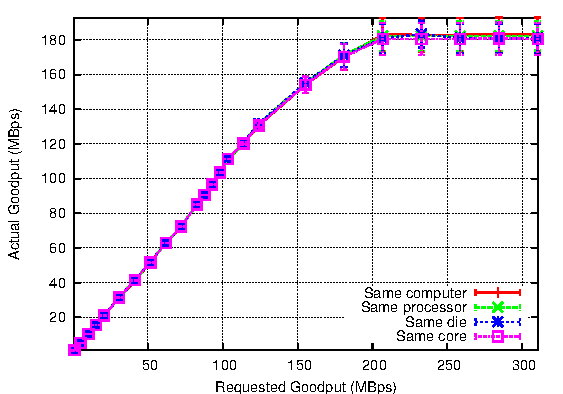
\includegraphics[height=0.65\columnwidth]{Graphs/intel/two_machines/requested_goodput_vs_actual_throughput}
    \end{center}
    \caption{Requested goodput versus actual goodput}
    \label{fig:goodputs}
\end{figure}

\begin{figure}[tb]
    \begin{center}
        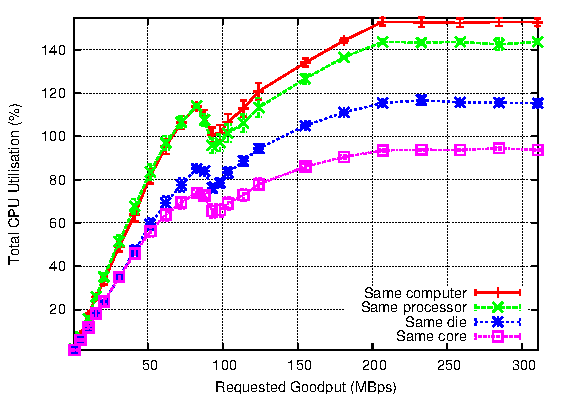
\includegraphics[height=0.65\columnwidth]{Graphs/intel/two_machines/requested_goodput_vs_cpu_total}
    \end{center}
    \caption{Total percentage of CPU consumed per core for different goodputs}
    \label{fig:cpuutil}
\end{figure}

A common measure of networking performance is \emph{goodput}, \emph{i.e.}, the number of bytes received by the application over a specific duration. Figure~\ref{fig:goodputs} shows the average achieved goodput versus the requested goodput (offered load) for the single connection scenarios discussed in the Section~\ref{sect:setup}. As the requested goodput increases, so does the actual goodput, until the system can not sustain the requested rate. It is worth noting that all tests peak at the same requested rate, indicating that the combinations of CPUs are not the bottleneck.

\begin{figure}[tb]
    \begin{center}
        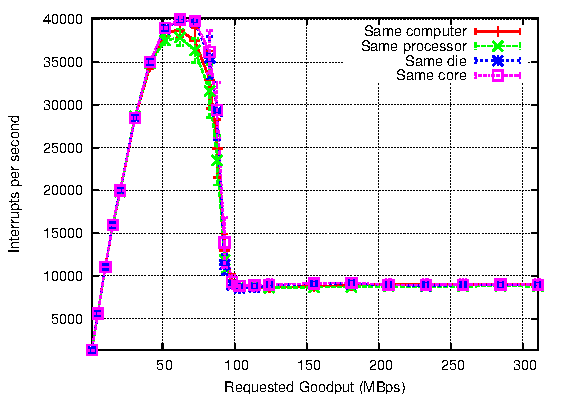
\includegraphics[height=0.65\columnwidth]{Graphs/intel/two_machines/requested_goodput_vs_intrpers}
    \end{center}
    \caption{Number of interrupts per second for a different goodputs}
    \label{fig:interruptspersecond}
\end{figure}

To investigate CPU usage, Figure~\ref{fig:cpuutil} shows the server's CPU utilisation versus the requested goodput. This figure is a sum of each core's percentage usage and, therefore, if two of the eight cores are 100\% utilised then a value of 200\% would be displayed.

It can be seen that the \emph{same core} scenario uses the least CPU cycles whilst achieving the same goodput as all other cases. Interestingly, the three cases which use two different cores exhibit different amounts of total CPU utilisation. This discrepancy is explained later by which resources each CPU shares.

In all cases Figure~\ref{fig:cpuutil} shows an increase in CPU utilisation until a requested goodput of roughly 80~MBps. Here, the CPU utilisation drops and later picks up. This is explained by Figure~\ref{fig:interruptspersecond} which displays the number of interrupts per second versus the requested goodput. The CPU utilisation drops when the number of hardware interrupts per second decreases. The reduction in interrupts is caused by Linux's interrupt mitigation technique, known as New-API (NAPI)~\cite{1268506}. NAPI disables network interrupts and polls the network adaptor. Interrupts are re-enabled when no more packets are available in the network adaptor, or there is no remaining buffer space within the network stack.

\subsection{CPU Caches}

%MF: AINA: Removed the table here since it doesn't add that much and we need the space.
%\begin{table}[tb]
%    \begin{center}
%        \begin{tabular}{|c|c|c|l|} \hline
%                             & Read Latency \\ \hline
%        L1 Data Cache        & 1.504 ns      \\ \hline
%        L2 Cache             & 7.054 ns     \\ \hline
%        Main memory (Sequential)    & 107.3 ns  \\ \hline
%        Main memory (Random) & 187.8 ns  \\ \hline
%        \end{tabular}
%    \end{center}
%    \caption{Memory read latencies as measured by LMbench}
%    \label{table:hardwarelookuplatency}
%\end{table}

Referring to Figure~\ref{fig:xeon} it can be seen that cores share different caches. Each core has its own L1 cache, and cores within the \emph{same die} share an L2 cache. If data is not in the local cache, the data must be copied from the cache a level above. This process repeats until data is found, or no level of the cache contains the data and it is requested from main memory. Main memory accesses are one order of magnitude slower than L2 accesses and two orders slower than L1 cache accesses. For example, in our system a single main memory access will take 187.8ns, a typical L2 cache access 7.054ns but a L1 data cache access only takes 1.504ns.

%Main memory accesses should be avoided as they are one order of magnitude slower than L2 cache accesses and two orders slower than L1 cache accesses.

Within this section, we show the cache miss rate for different levels of the cache hierarchy versus the requested goodput. The cache miss rate is the number of cache lines which are fetched in to that cache divided by the number of completed instructions. Completed instructions which do not touch memory are also counted. Thus, the cache miss rate may be higher than shown. A high value for this metric indicates the cache is not being utilised well and therefore spends time fetching from a higher cache level or main memory.

\begin{figure}[tb]
    \begin{center}
       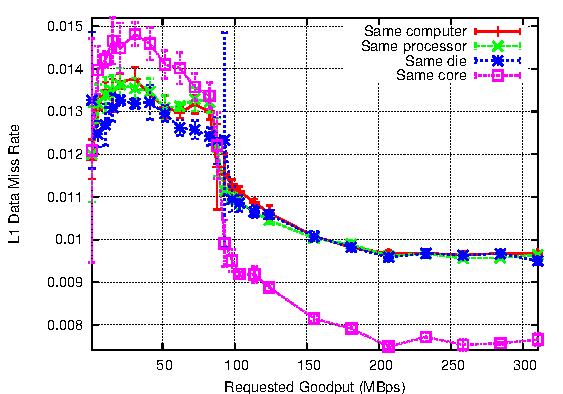
\includegraphics[height=0.65\columnwidth]{Graphs/intel/two_machines/requested_goodput_vs_L1_MISS_RATE}
    \end{center}
    \caption{Level 1 cache miss rate for different goodputs}
    \label{fig:l1cacherate}
\end{figure}

\emph{Same core} has the lowest CPU utilisation. One reason for this can be seen in Figure~\ref{fig:l1cacherate} which shows the L1 data cache miss rate. As the SoftIRQ and server application are executed on the same core, packet data will reside within the L1 cache and, therefore, the L1 will be utilised more efficiently. Because the hardware architecture does not allow the other combinations of cores to share an L1 cache there is a higher L1 miss rate. As expected these combinations all have a similar miss rate.

\begin{figure}[tb]
    \begin{center}
       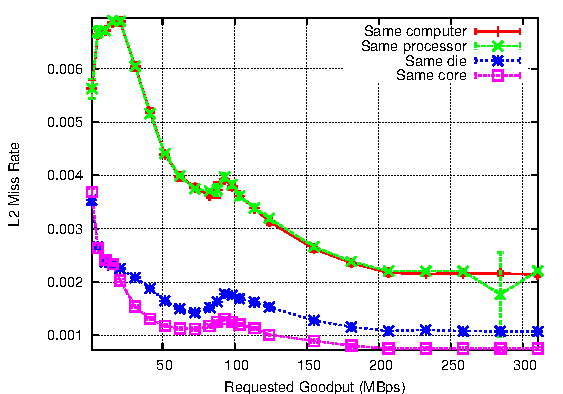
\includegraphics[height=0.65\columnwidth]{Graphs/intel/two_machines/requested_goodput_vs_L2_MISS_RATE}
    \end{center}
    \caption{Level 2 cache miss rate for different goodputs}
    \label{fig:l2cacherate}
\end{figure}

The next lowest CPU utilisation is observed in the \emph{same die} case. This is caused by the two cores sharing an L2 cache. Sharing the L2 cache allows the \emph{same die} to avoid reading and writing to main memory. This is shown by a lower L2 miss rate in Figure~\ref{fig:l2cacherate}.

The final two cases are \emph{same processor} and \emph{same computer}. Neither of these cases share any level of cache and thus have similar miss rates as again seen in Figure~\ref{fig:l1cacherate} and Figure~\ref{fig:l2cacherate}. Therefore, there must be another reason for the discrepancy in CPU utilisation shown in Figure~\ref{fig:cpuutil}.

\subsection{Front Side Bus}
\begin{figure}[tb]
    \begin{center}
       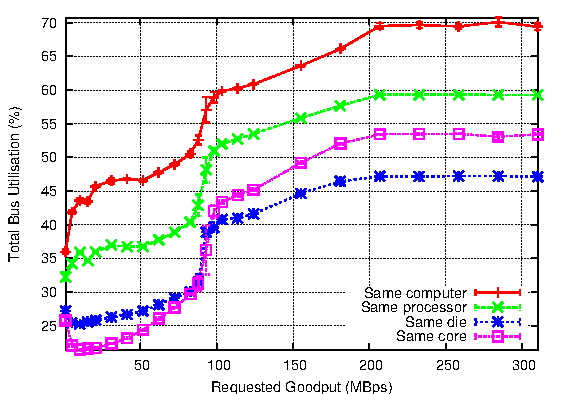
\includegraphics[height=0.65\columnwidth]{Graphs/intel/two_machines/requested_goodput_vs_BUS_UTIL}
    \end{center}
    \caption{Front Side Bus Utilisation}
    \label{fig:FSBUtilisation}
\end{figure}

The \emph{same processor} and \emph{same computer} combinations do not have any shared cache, yet their performance differs. This can be attributed to additional front side bus (FSB) traffic, as shown in Figure~\ref{fig:FSBUtilisation}. To ensure that the memory locations stored in each core's cache are coherent, Intel uses the MESI protocol~\cite{808204}. This requires messages to be broadcast over the FSB to all other cores, for each main memory read or write. On each write request, other cores must invalidate any locally cached copies of the written location. On reads from main memory, the other cores may opportunistically reply on behalf of the main memory if the read location exists in their cache. These coherency messages account for most of the bus traffic.

Recalling Figure~\ref{fig:xeon}, there are two front side buses (FSBs) in our test machines, one for each processor. These buses are connected via the Northbridge (in our case the Intel 5000X MCH chipset) which serves as an arbiter for main memory and other devices. Typically the Northbridge will forward all broadcasts from one FSB to the other, but, to minimise traffic, the Intel 5000X MCH includes a \emph{snoop filter}. The snoop filter keeps track of which memory locations are cached behind each FSB and filters the traffic appropriately therefore not forcing the processor to response to unnecessary snoop requests. This filtering reduces the FSB traffic by 10\% when both cores share a bus and therefore allows the CPU to be more efficiently utilised.
%, and thus decreases overall CPU utilisation by 10\%.

%%%L1 Instruction cache miss rate > L1 Ccahe miss rate -this implies you need a bigger L1 Instruction cache then L1 data cache - We've not included this

\subsection{Multiple Connections}
\label{sect:multipleconnections}

All previous experiments used a single server with one TCP connection between the machines. We now extend these experiments to use four network adaptors on each machine, connecting them with point-to-point links. One machine creates four servers whilst the other four clients. TCP connections are then established between the clients and servers and data sent at specific bit rates. The reason for this second experimental setup is two-fold. Firstly, using four cards we can examine the bottlenecks shown in the previous section using higher throughput. Secondly, with the extreme cost of 10GbE network cards, at the time this experiment was performed, many server administrators may attempt to increase network throughput by using many, cheaper, 1GbE cards and thus this scenario is likely to occur in reality.

In all scenarios the interrupts, and thus the network protocol processing for all four adaptors, were assigned to a single core. The core on which the servers are executed was decided by the type of scenario. We use the same set of scenarios as the previous experiments, \emph{i.e.} \emph{same core}, \emph{same die}, \emph{same processor} and \emph{same computer}.


\begin{figure}[tb]
    \begin{center}
      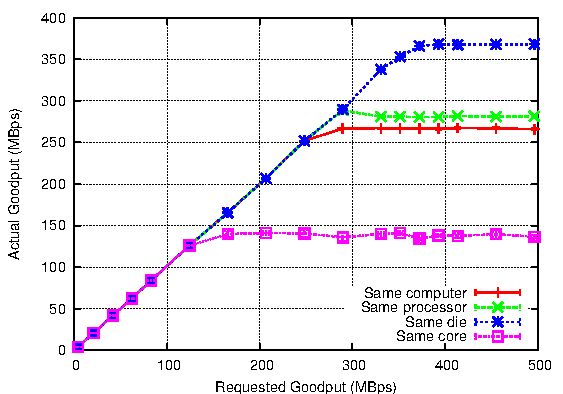
\includegraphics[height=0.65\columnwidth]{Graphs/intel/two_machines/4_connections/requested_goodput_vs_actual_throughput}
    \end{center}
    \caption{Requested goodput versus actual goodput for multi-connection tests}
    \label{fig:multigoodputs}
\end{figure}

\begin{figure}[tb]
    \begin{center}
      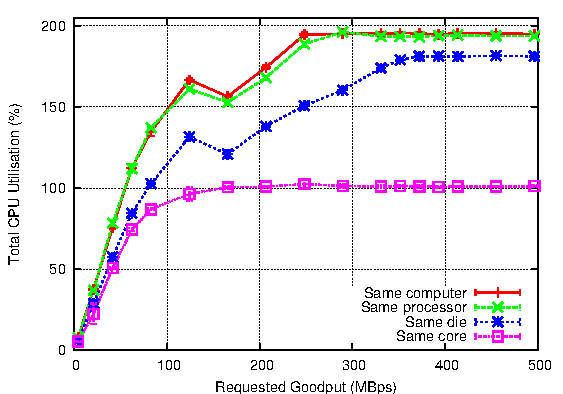
\includegraphics[height=0.65\columnwidth]{Graphs/intel/two_machines/4_connections/requested_goodput_vs_cpu_total}
    \end{center}
    \caption{Total percentage of CPU consumed per core for different goodputs for multi-connection tests}
    \label{fig:multicpuutil}
\end{figure}

\begin{figure}[tb]
    \begin{center}
      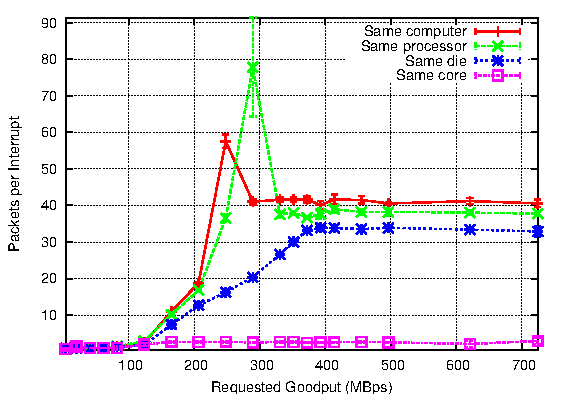
\includegraphics[height=0.65\columnwidth]{Graphs/intel/two_machines/4_connections/requested_goodput_vs_pktsperint}
    \end{center}
    \caption{Requested goodput versus number of interrupts per packet}
    \label{fig:pktsperinter}
\end{figure}

\begin{figure}[tb]
    \begin{center}
      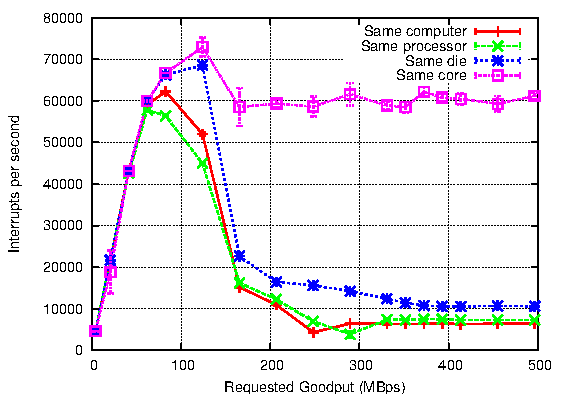
\includegraphics[height=0.65\columnwidth]{Graphs/intel/two_machines/4_connections/requested_goodput_vs_intrpers}
    \end{center}
    \caption{Requested goodput versus interrupts per second for multi-connection tests}
    \label{fig:multiintrpers}
\end{figure}

Recalling the single TCP connection experiments, all scenarios achieved the same maximum throughput. However, in the multiple connection experiments, no scenarios reached the network's maximum throughput. We can see from Figure~\ref{fig:multigoodputs} and Figure~\ref{fig:multicpuutil} that the maximum goodput is limited by the CPUs becoming fully utilised. The \emph{same die} scenario attains the best goodput because of the benefits of the L2 cache. There was a 10~MBps difference between the \emph{same processor} and \emph{same computer} scenarios. This difference is again to attributed to a lower bus utilisation. Finally, the \emph{same core} scenario is the worst, reaching only 40\% of the goodput of the \emph{same die} scenario.

Clearly, a single core could not process packets at a fast enough rate. Interestingly, the maximum rate the \emph{same core} scenario did achieve was 15\% lower than in the single connection experiments. Figure~\ref{fig:pktsperinter} and Figure~\ref{fig:multiintrpers} explains this decrease. Recall that as the number of packets per second increases, so does the number of interrupts. Eventually, Linux's interrupt mitigation technique begins to poll the adaptor to reduce the number of interrupts. Figure~\ref{fig:multiintrpers} shows that in all except the \emph{same core} scenario the interrupts are mitigated.

Figure~\ref{fig:pktsperinter} shows the average number of packets received per interrupt versus request rate. In the two-core scenarios between 30 and 40 packets were received per interrupt. However, the \emph{same core} scenario managed only 2 packets per interrupt. Recall that when using interrupt mitigation, the network stack will receive packets until there are none remaining in the network adaptor or the network stack's receive buffer is full. We noted in the \emph{same core} scenario that the application could not remove data from this buffer faster than the packets arrived. This is because the application is continually context switched by a higher priority interrupt. In contrast, the applications in the two-core scenarios were able to consume the buffer faster than it was filled. This is because the interrupt handling was not executed on the application's core and thus fewer context switches occurred.

%Figure~\ref{fig:pktsperinter} shows the average number of packets received per interrupt versus request rate. In the two-core scenarios between 30 and 40 packets were received per interrupt, however, the \emph{same core} scenario managed only 2 packets per interrupt. Recall that interrupt mitigation will receive as many packets as available in the network adaptor or until the network stack's receive buffer is full. We noted in the \emph{same core} scenario that the application could not remove data from this buffer faster than the packets arrived. This was a result of the application continually being context-switched by a higher priority interrupt. In contrast, the applications in the two-core scenarios were able to consume the buffer faster than it was filled. This was because the interrupt handling was not executed on the application's core and, thus, fewer context switches occurred.


\subsection{Locks}
\label{sect:locks}

Linux's \emph{lockstat} was used to record many different operating system locking metrics including \emph{wait time}.  Wait time is how long a task waits before acquiring a lock. A higher value indicates that the shared data or device is highly contended for. We find that in the absolute worst case in any of the experiments, the effect of waiting for locks is less than 0.02\% of the experiment duration. This suggests that the Linux networking stack has been optimised for concurrent access in our experimental workload.

\subsection{Summary}
\label{sect:sum}
Using a single core to process both the application and network code is the optimal solution for lower throughputs. As the number of packets per second increases, a single core cannot process packets fast enough and therefore two cores should be used. We show that using two cores changes the performance dramatically. The best pairs of cores are those which share the fastest resources, for example, the level 2 cache.
%%Can you, from the experimental results, be more explicit about which two-core configuration to use?

\section{Discussion and Future Work}
\label{sect:future_work}
This paper presents evaluation of network protocol processing using a particular multicore architecture and operating system. We, however, feel that our results can be generalised to other architectures running different operating systems. This is true because most operating systems use the same concept of interrupts and differed processing (SoftIRQ). Additionally, SMP systems share similar architectures such as CPU caches, buses and shared memory.

Recently SMP architectures have been changing with the introduction of Non-Uniform Memory Architectures (NUMA). Traditionally SMP machines use a Uniform Memory Architecture (UMA). In a UMA there is a one shared memory controller to access all of main memory. As we have shown in this paper accessing main memory is relatively slow. To address this caches are placed near the CPU to reduce the number of main memory requests. However, as programs and operating systems increase their memory footprint the size of caches also needs to increase. An alternative memory architecture is NUMA where the main memory is partitioned in to multiple regions each being accessed exclusively by a different memory controller. Typically, each core has one memory controller assigned to it which provides fast access to that region. However, accessing the memory regions assigned to other cores is costly. Therefore work is needed to evaluate the network protocol performance of NUMA architectures.

Throughout our experiments, we have combined two or more gigabit-per-second (Gb/s) network adaptors to simulate higher speed networks. Our tests will be made against 10 Gb/s hardware adaptors as they become more ubiquitous. These adaptors may reduce the CPU load by implementing greater levels of interrupt mitigation.

Whilst this study highlights the number of bottlenecks that exist for network protocol processing within a multicore environment, it has not yet addressed two important questions: how can the knowledge of the different bottlenecks be used to design faster and more efficient networked systems, and how does this work apply to other research efforts. Used in conjunction with other techniques such as RSS~\cite{RSS} the results of this paper could be used to design an adaptive network scheduler which forces the application and network protocol processing to take place on the most appropriate core(s). For example, deciding whether to use one or more cores is an important consideration in modern servers where power consumption is a major cost. Our results show that when network throughput demand is less than 1.5GB/s, a single core is more than adequate and therefore the network scheduler should use RSS to force the network protocol processing and application processing to take place on the same core.

The experiments within this paper are a first step to understanding the bottlenecks within an end-host. To perform this analysis we use a point-to-point network and over a limited number of connections. As part of future work, we plan on evaluating the network protocol processing performance when many connections are used. This type of analysis is essential for large servers.

%MF: AINA: Do we really need to talk about jumbo frames? Afterall, i don't see it making MUCH of a difference and we need the space in this paper
%In our experiments, we used the standard Ethernet maximum transmission unit (MTU) size of 1500 bytes. Future networks may use jumbo frames, which increase the MTU to 9000 bytes~\cite{jumbo}. Increasing the MTU size allows more data to be sent per packet and therefore may result in fewer network interrupts, decreasing CPU utilisaton. Thus we plan to examine how jumbo frames may affect overall network protocol processing performance.

%We also plan to investigate processing smaller message sizes. Small  message sizes may require the CPU to do more overall protocol processing for the same amount of data as well as potentially increasing the number of interrupts causing higher CPU usage.

\section{Conclusions}
\label{sect:conclusion}

In this paper we have shown the effects of executing application and network processing on different cores within a multi-core system. We show that due to advantages gained by L1 caches, executing both the application and network processing on the same core is sufficient to support transfer rates of up to 1.5GB/s. Moreover, using more than one core is detrimental because it actually increases the total CPU utilisation without increasing the transfer rate.

With higher transfer rates one core can no longer process packets fast enough and therefore a pair of cores is needed. In this pair, one of these cores should be used for the application processing and the other for the network processing. Performance of different pairs of cores vary depending on whether they share resources such as caches.  Thus choosing the right pairs of cores to execute application and network code is important.  We have shown that choosing the wrong pair of cores can decrease performance by over 40\%.  This figure is likely to increase as systems incorporate a higher number of cores.

\bibliographystyle{IEEEtran}
\bibliography{cachehits}

\end{document}

